\subsection{User Interfaces}
The application in use by the customer will let the user line up, book a visit, and view the details about the queue or the booked visit.
The web application in use by the store manager will let him view store information and statistics. The employee will use the web application to line up on behalf of visitors, to call them, to check entrances, and report exits. Functional requirements are fully described in the next subsection. 

The following mockups represent a basic idea of what the mobile app and the web app will look like.

\begin{figure}[H]
    \begin{minipage}[b]{8cm}
    \centering
    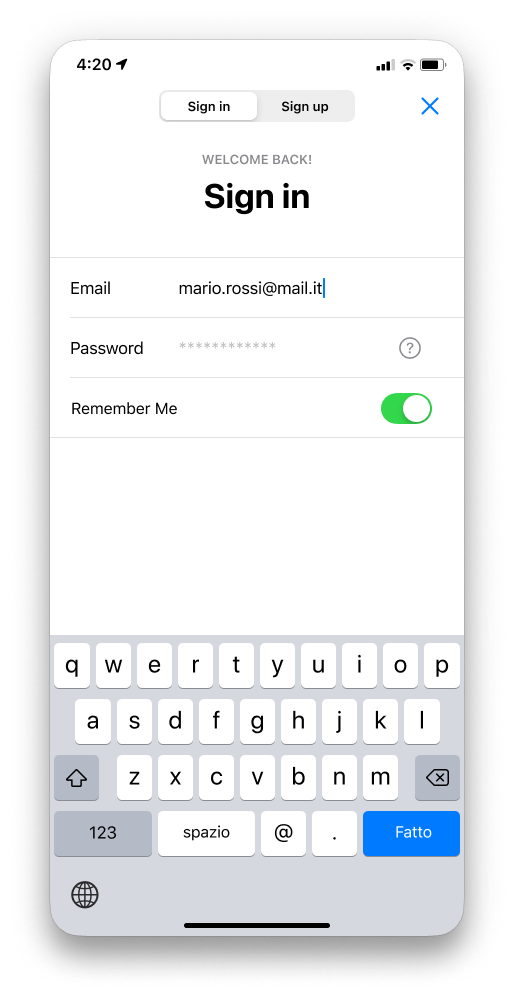
\includegraphics[width=6cm]{AppLogIn.png}
    \caption{Sign in}
    \end{minipage}
    \ \hspace{2mm} \hspace{3mm} \
    \begin{minipage}[b]{8cm}
    \centering
    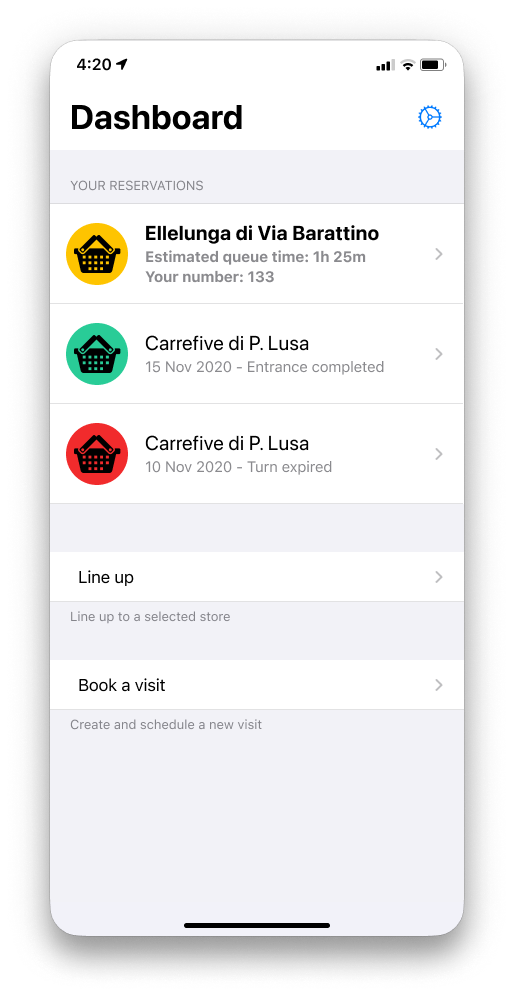
\includegraphics[width=6cm]{AppDashboard.png}
    \caption{App dashboard}
    \end{minipage}
\end{figure}

\begin{figure}[H]
    \centering
    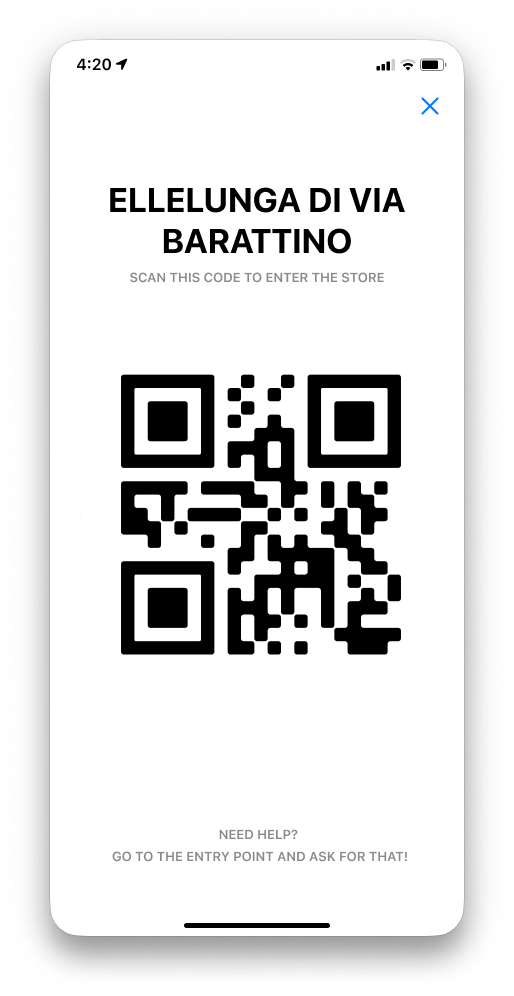
\includegraphics[width=6cm]{AppQRCode.png}
    \caption{QRCode to be scanned}
\end{figure}

\begin{figure}[H]
    \centering
    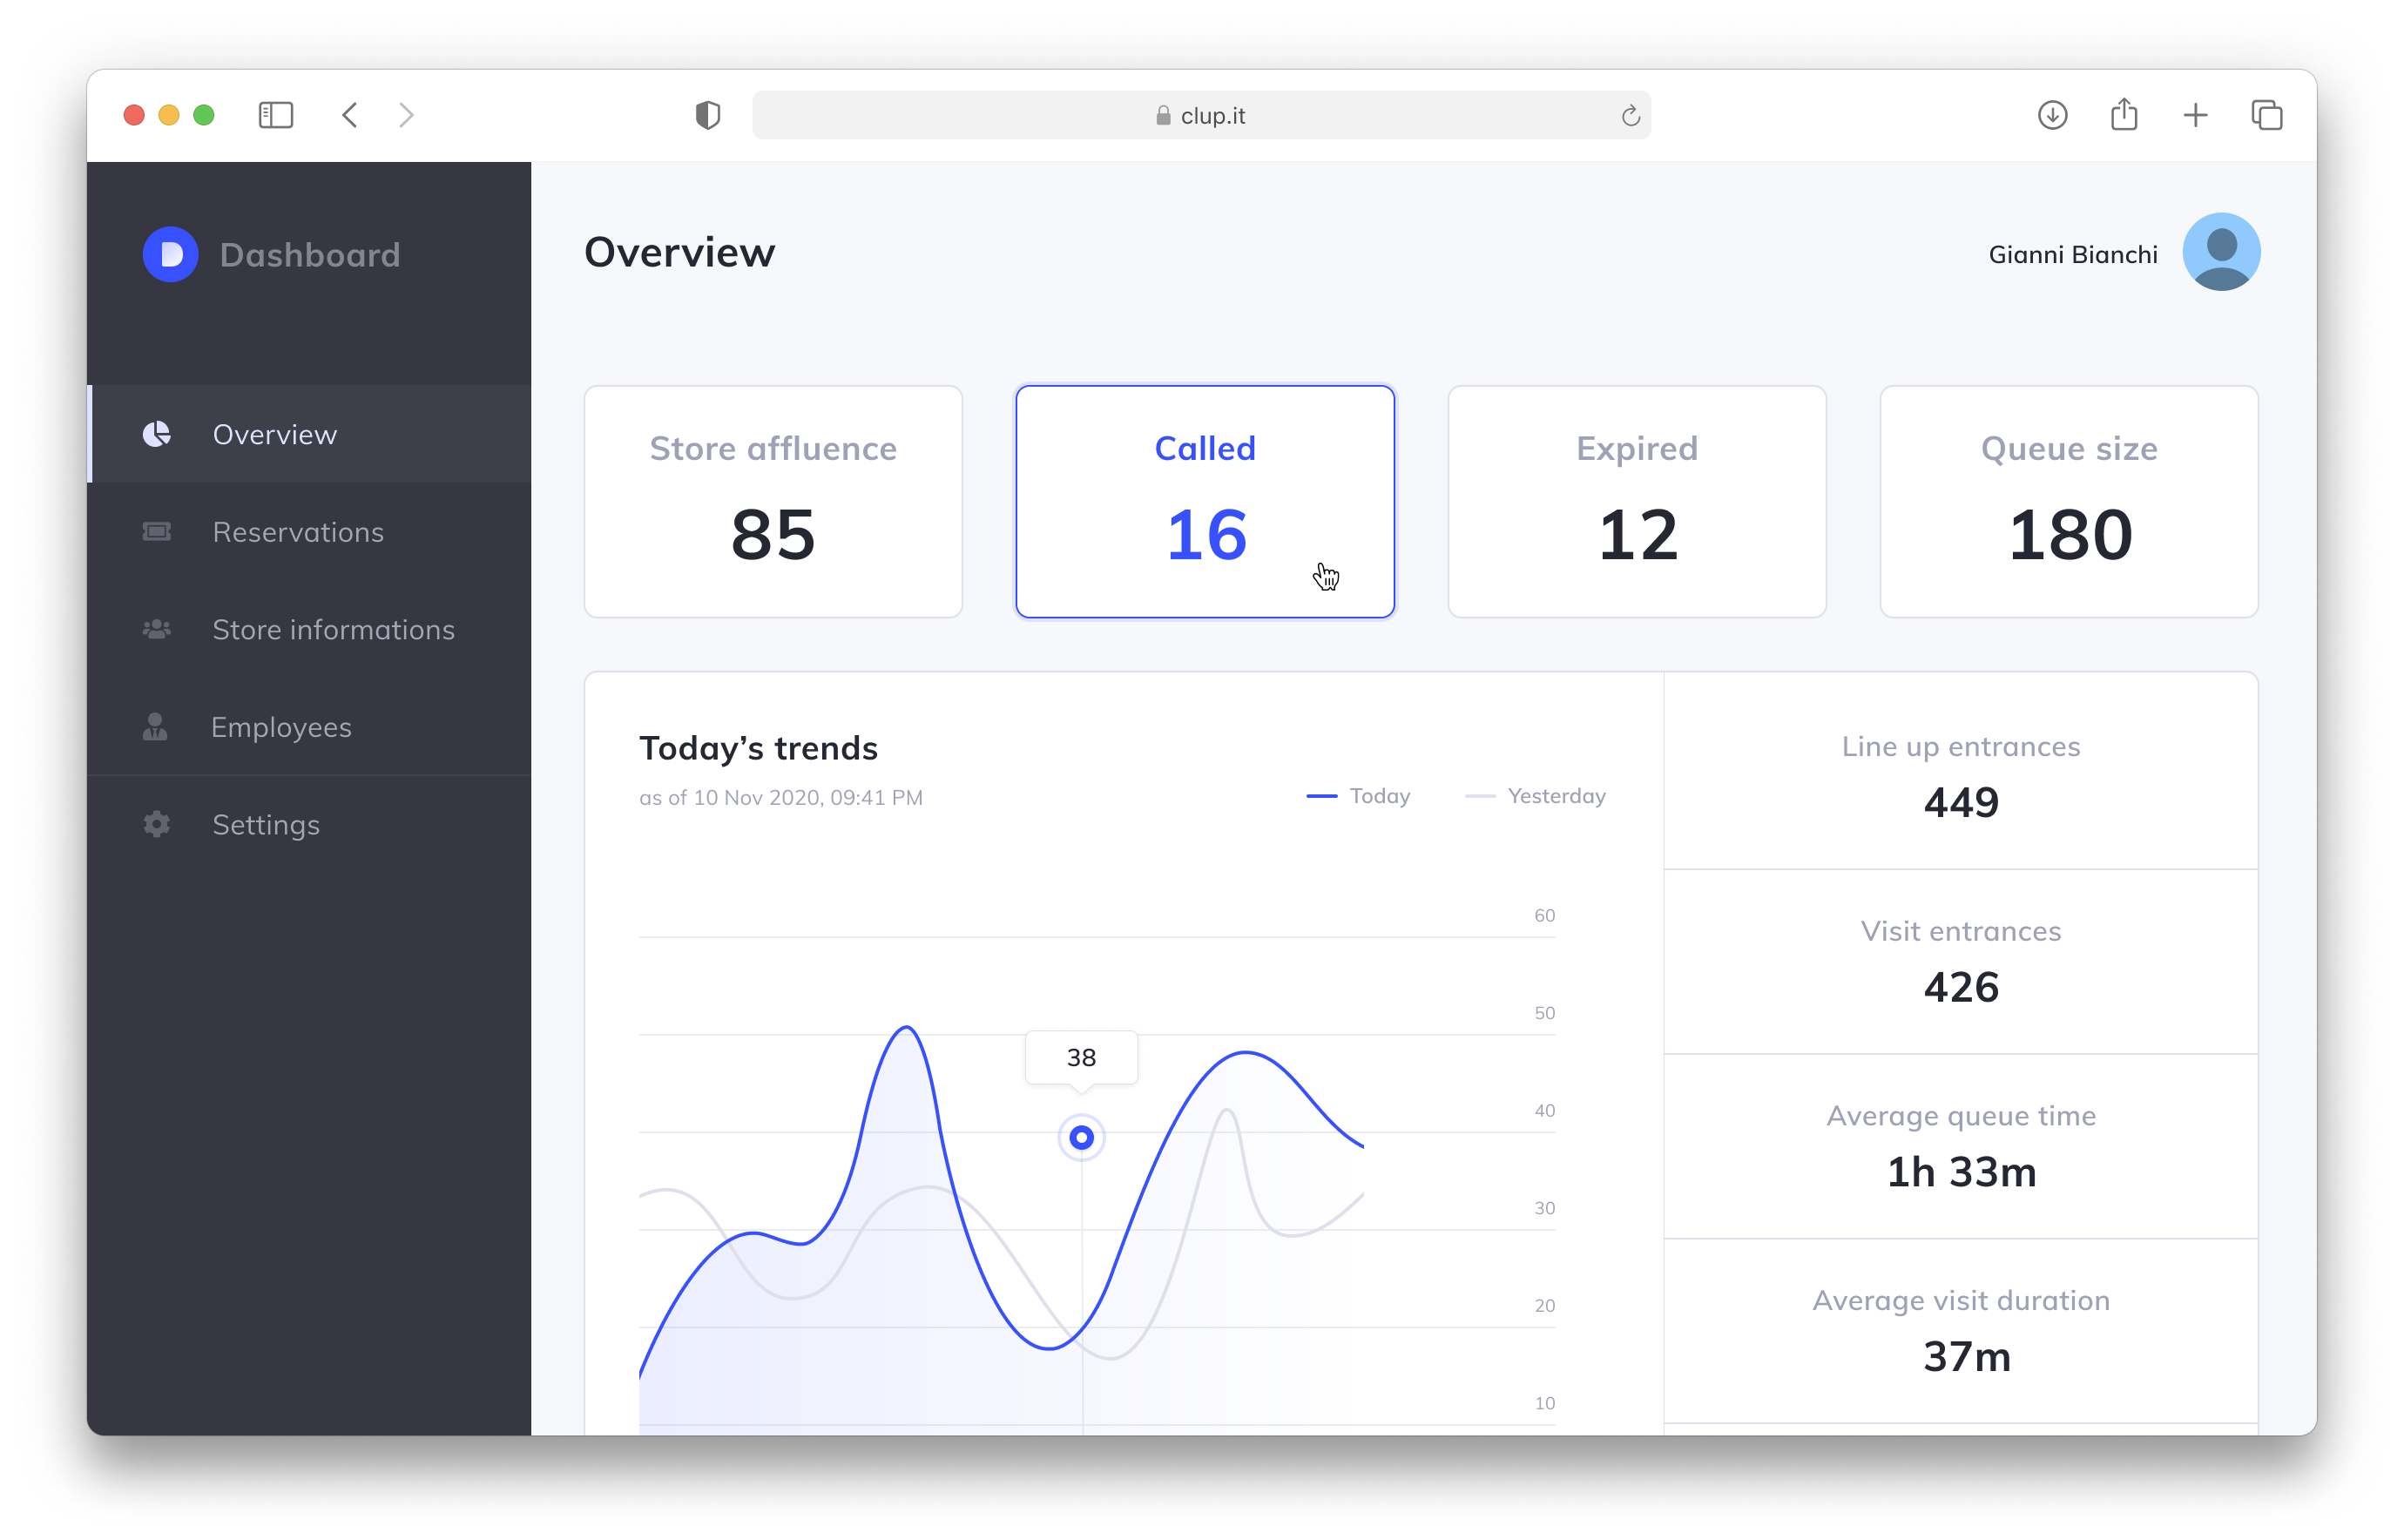
\includegraphics[width=16cm]{WebAppDashboard.png}
    \caption{Web application dashboard}
\end{figure}

\begin{figure}[H]
    \centering
    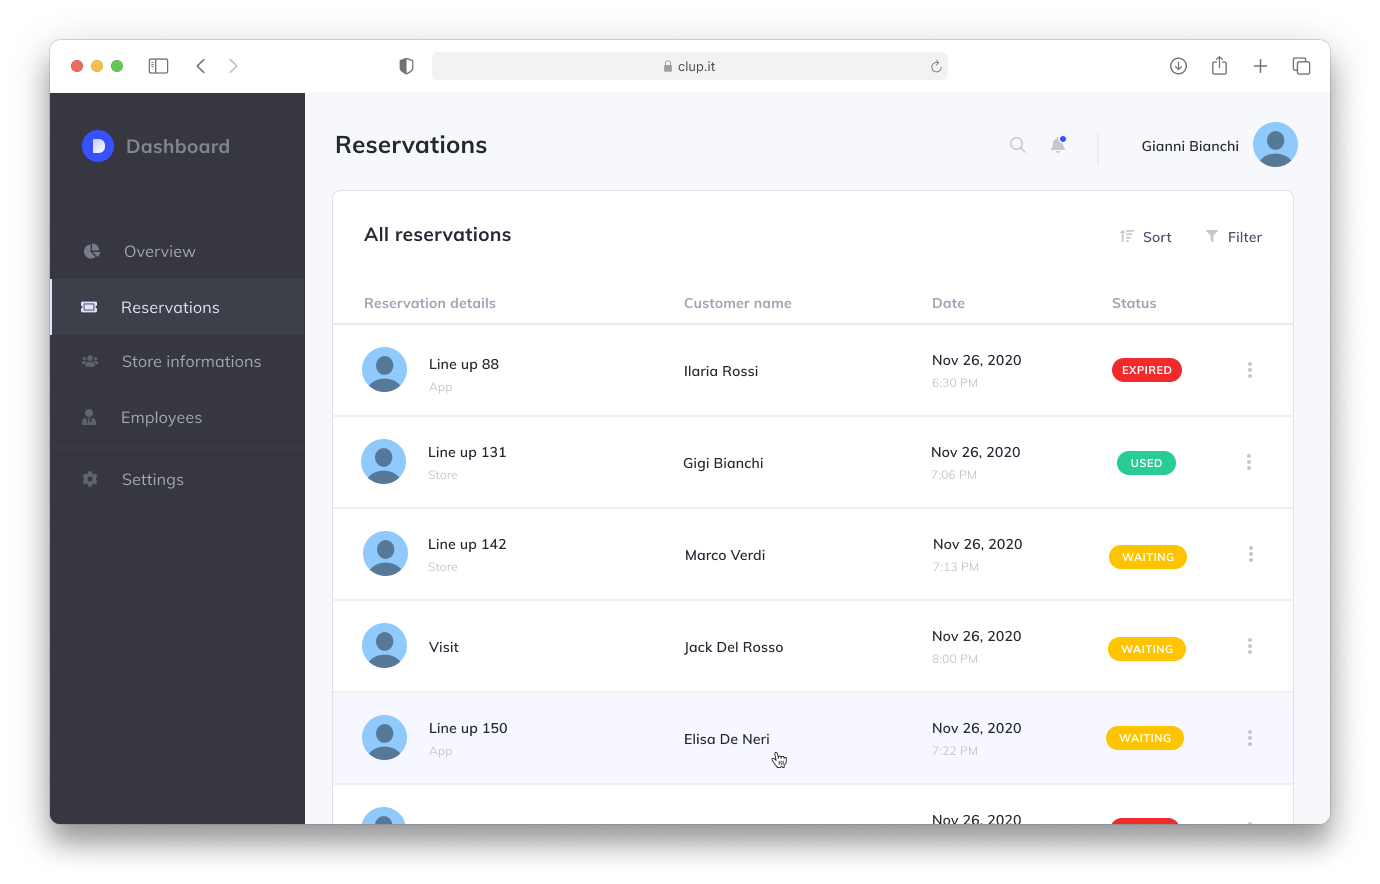
\includegraphics[width=16cm]{WebAppReservations.png}
    \caption{Web application reservations page}
\end{figure}
Other mockups related to other parts of the applications will be available in the design document

\subsection{Hardware Interfaces}
\label{hardware interfaces}
The CLup applications interact with three types of actors and two of them share the same hardware requirements:
\begin{itemize}
    \item Regarding the customer: he/she needs an iOS/Android smartphone with a working Internet connection and GPS sensor. The application will not require a lot of computational power, therefore any recent (last couple of years) smartphone will be suitable.
    \item Regarding the store manager and the employees: he/she needs a modern web browser and an Internet connection. The web application will run easily on any desktop computer of the last decade.
\end{itemize}

\subsection{Software Interfaces}
The system will use the following external software interfaces:
\begin{itemize}
    \item \textbf{Public geodata provider:} the system will connect to a public geodata service API (like Google Maps or OpenStreetMap and the like) to compute a route from the user's location to the grocery store and in particular to retrieve an estimated travel time
    \item \textbf{Android/iOS system APIs:} the mobile application will be developed for iOS and Android, therefore it will interact with the underlying system's primitives.
\end{itemize}

\subsection{Communication Interfaces}
The mobile application and the web application will communicate with CLup via an internet connection.